\subsection{System Model}
Figure~\ref{fig:wsn} depicts the structure of a WSN used in our model. We consider a WSN as an undirected graph \(G=(V,E))\), where \(V=\{v_1, v_2, \ldots, v_N\}\) is the set of \(N\) sensor nodes and \(E \subseteq V \times V\) represents bidirectional communication links between neighboring nodes. Each node \(v_i\) is equipped with a sensing modality and generates a time-series measurement \(x_i(t)\) at discrete time steps \(t=1, 2, \ldots, T\). Communication between \(v_i\) and \(v_j\) is possible if \((v_i,v_j) \in E\).

\begin{figure}
\centering
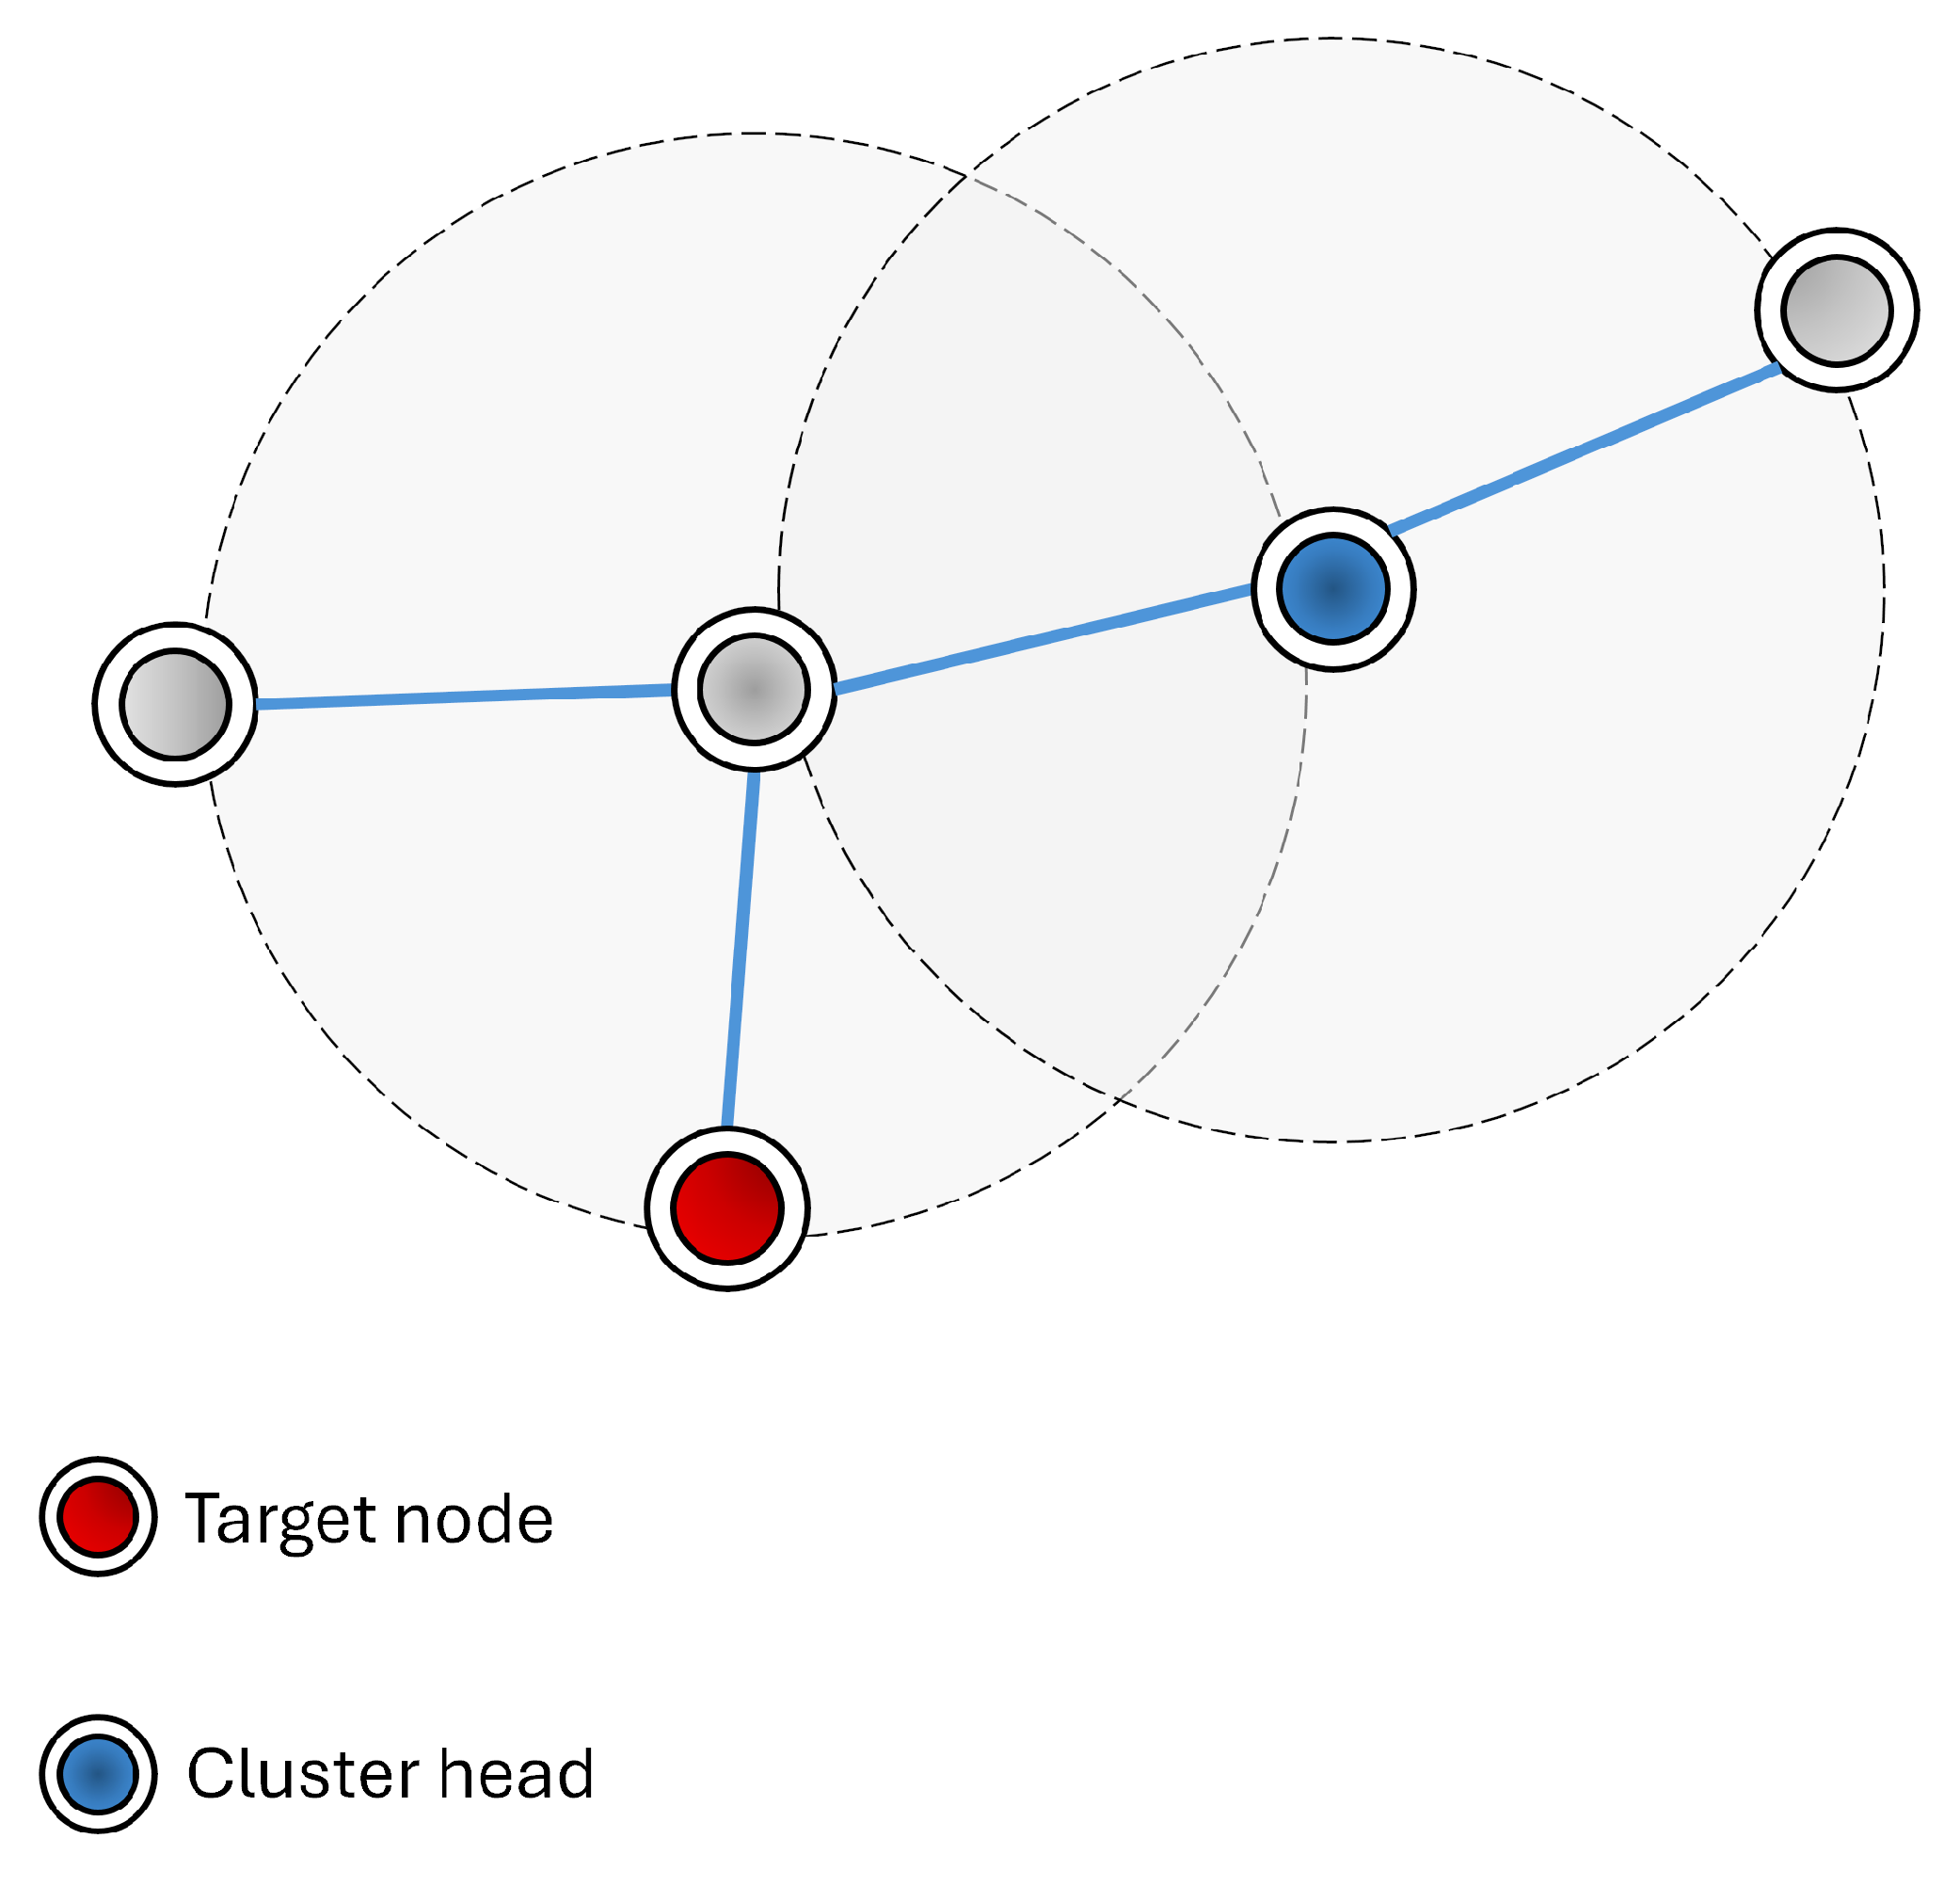
\includegraphics[width=0.8\linewidth]{images/WSN.png}
\caption{Example of a WSN cluster with a base station. Target node is the node which data sequence needed fault classification.}
\label{fig:wsn}
\end{figure}

This paper make the following additional assumptions:
\begin{itemize}
\item Static or Slowly Varying Topology: Sensor nodes are assumed to be stationary or exhibit negligible mobility during the diagnosis window, so that network links \(E\) remain constant or change infrequently.
\item Global Time Synchronization: Nodes maintain loosely synchronized clocks, ensuring measurements \(x_i(t)\) across the network align within a bounded jitter.
\item Existence of a Single High-Capacity Node/Sink: A base node with higher computation and memory resources is reachable (directly or multi-hop) from all nodes and knows the network topology apriori.
\end{itemize}

\subsection{Fault Taxonomy}
\label{subsec:types}
Building upon the general categorization of faults, this section details the specific characteristic-based fault types that are the focus of our detection and diagnosis efforts. These faults represent common anomalies observed in WSN sensor readings and are well-documented in the literature \cite{Saeed2021, Hasan2024, Shi2024, Ni2009}. Understanding their distinct signatures is essential for designing robust fault detection and classification algorithms. The faults considered in this study are: hardover, drift, spike, erratic, and stuck-at fault.

\subsubsection{Hardover Fault}
A hardover fault, also commonly referred to as a bias fault, occurs when the sensor's output signal experiences a sudden and persistent shift by a constant offset from its normal operational range \cite{Saeed2021, Shi2024, Hasan2024}. The sensor continues to respond to changes in the measured variable, but all readings are offset by this fixed amount. This can be caused by issues like calibration errors or a sudden change in the sensor's baseline. If \(S_\text{normal}(t)\) is the true sensor reading at time \(t\), the faulty signal, \(S_\text{hardover}(t)\), can be represented as:
\begin{equation}
S_\text{hardover}(t) = S_\text{normal}(t) + b,
\label{eq:hardover}
\end{equation}
where \(b\) is a constant bias value \cite{Saeed2021}.

\subsubsection{Drift Fault}
A drift fault is characterized by a gradual and continuous deviation of the sensor readings from the true values over time \cite{Saeed2021, Hasan2024}. This deviation often manifests as a linear increase or decrease, though non-linear drifts are also possible. Drift can be caused by aging components, environmental changes affecting the sensor, or gradual degradation of sensor calibration. For a linear drift, the faulty signal, \(S_\text{drift}(t_n)\) at discrete time sample \(n\), can be modeled as:
\begin{equation}
S_\text{drift}(t_n) = S_\text{normal}(t_n) + n \cdot b_0,
\label{eq:drift}
\end{equation}
where \(n\) is the time index or sample number, and \(b_0\) is an initial constant drift rate \cite{Saeed2021}. Hasan et al. also model this as \(S_\text{drift}^N = S_\text{normal}^N +\beta^N\), where \(\beta^N\) represents the accumulated drift \cite{Hasan2024}.

\subsubsection{Spike Fault}
Spike faults are transient anomalies characterized by sudden, short-duration, large-magnitude deviations in sensor readings, after which the readings typically return to normal or near-normal values \cite{Saeed2021, Shi2024}. They appear as sharp peaks or impulses in the data stream. Spikes can be caused by electromagnetic interference, power supply glitches, or other transient disturbances. If \(S_\text{normal}(t)\) is the normal signal, a spike at time \(t_s\) might be represented as:
\begin{equation}
S_\text{spike}(t_s) = S_\text{normal}(t_s) + b_\text{spike},
\label{eq:spike}
\end{equation}
where \(b_\text{spike}\) is a constant large value, and for \(t \neq t_s\): \(S_\text{spike}(t) \approx S_\text{normal}(t)\) \cite{Saeed2021, Shi2024}.

\subsubsection{Erratic Fault}
An erratic fault, sometimes referred to as precision degradation or increased noise, is characterized by sensor readings that exhibit random fluctuations of significantly increased amplitude around the true value \cite{Saeed2021}. While the average reading over a long period might still be close to the true value, the individual readings become highly unreliable due to the increased variance. This can be caused by failing sensor components, loose connections, or severe environmental interference. The faulty signal can be represented as:
\begin{equation}
S_\text{erratic}(t) = S_\text{normal}(t) + \eta(t),
\label{eq:erratic}
\end{equation}
where \(\eta(t)\) is a noise term with zero mean but significantly higher variance (\(\sigma_\text{erratic} \gg \sigma_\text{normal}\)) than the inherent sensor noise under normal operating conditions \cite{Saeed2021}.

\subsubsection{Stuck-at Fault}
A stuck-at fault (or stuck fault) occurs when the sensor output remains fixed at a constant value for a prolonged period, irrespective of any changes in the measured physical phenomenon \cite{Saeed2021, Hasan2024, Shi2024}. This constant value could be zero, a previous valid reading, the maximum or minimum of the sensor's range, or an arbitrary value. Common causes include complete sensor failure, signal clipping, or a disconnection in the data path. Mathematically, this is expressed as:
\begin{equation}
S_\text{stuck} = c,
\label{eq:stuck}
\end{equation}
where \(c\) is a constant value, either from the nearest normal value or a random value \cite{Saeed2021, Hasan2024, Shi2024}.

% TODO: add sample figure for each fault types

\subsection{Problem Statement}
Given a segment of a sensor time series and a predefined set of fault classes, the problem is to assign the most appropriate fault class label to that time series segment.

Consider an input time series \(X_w = (x_t, x_{t+1}, \ldots, x_{t+w-1})\) of length \(w\), where \(x_i \in \mathbb{R}\) is the sensor reading at discrete time step \(i\). Define \(C = \{c_1, c_2, \ldots, c_K\}\) as the set of \(K\) mutually exclusive fault classes as detailed in the fault taxonomy in Section~\ref{subsec:types} and the normal (fault-free) class.

The object is to learn a classification function (or hypothesis) \(h\) that maps the input feature vector \(\mathbf{x}\) (derived from \(X_w\)) to a predicted fault class label \(\hat{y}\ \in C\).
